\pagebreak
\newgeometry{margin=11mm}
\pagenumbering{gobble}

\vspace*{\fill}
\begin{center}
    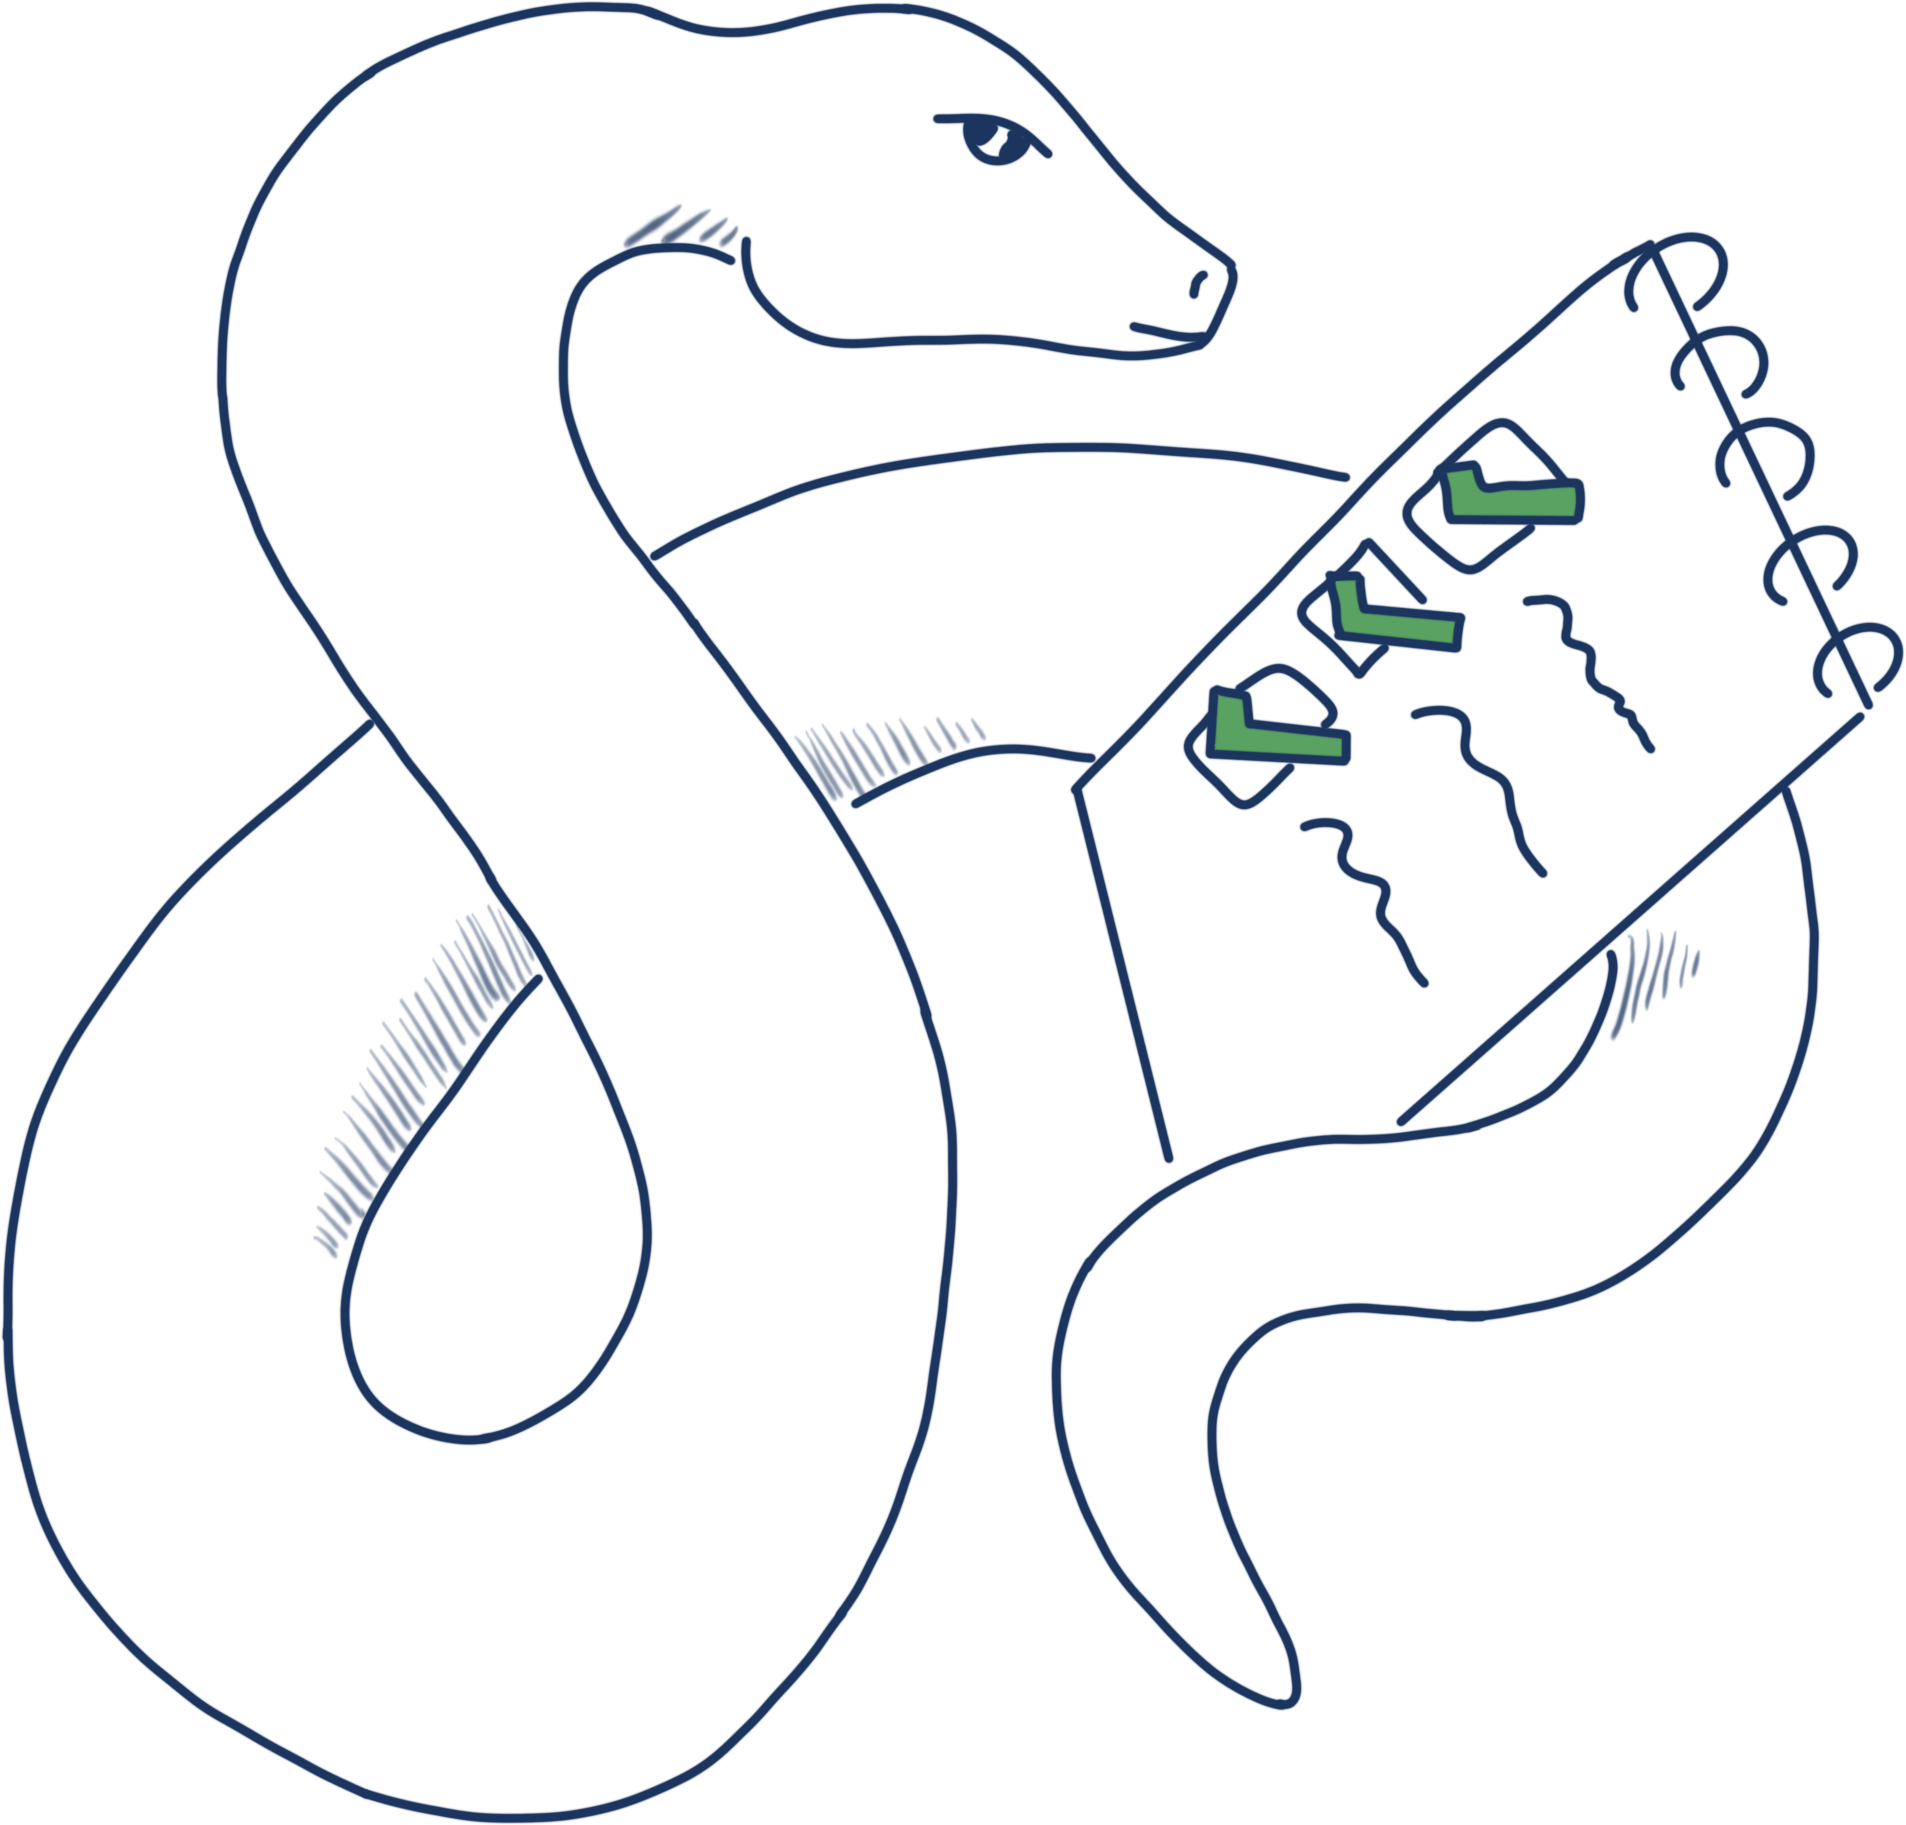
\includegraphics[width=.9\linewidth]{img/illustrations/about-testing.png}
\end{center}

\vfill
\begin{tabular}{cll}
    \faCodeBranch{}         & v1.2-dev                                                            &                                                                                                          \\[1em]
    \faCreativeCommons{}    & \faCreativeCommonsBy{} \faCreativeCommonsNd{} \enspace CC BY-ND 4.0 &                                                                                                          \\
    \faCopyright[regular]{} & 2026 Freya Bruhin                                                   &                                                                                                          \\
    \faPaintBrush{}         & Illustrations by Tony Maier                                         &                                                                                                          \\[1em]
    \faGithub{}             & The-Compiler/pytest-quick-ref                                       & \hspace{2.5em}\multirow{2}{5em}{\qrcode[height=4.25em]{https://github.com/The-Compiler/pytest-quick-ref}} \\
    \faFilePdf{}            & https://pyte.st/ref.pdf                                             &                                                                                                          \\[1em]
    \faEnvelope{}           & freya@bruhin.software
\end{tabular}

\restoregeometry
